\documentclass[UTF8]{report}
\usepackage[margin=0.5in]{geometry}
\usepackage{graphicx}
\usepackage{xetexko}

\title{%
    <컴퓨터프로그래밍 3> 실습 보고서 \\
    \large [제 09 주] 스택}
\author{201704150 허강준}
\date{\today}

\begin{document}
    \maketitle
    \tableofcontents

    \chapter{프로그램 설명서}
        본 보고서에서는 스택을 정의 및 구현하고 이를 응용하여 여러 데이터를 삽입/삭제 처리하는 프로그램에 대해 기술한다.

        \section{프로그램의 전체 설계 구조 (MVC 등)}

            \paragraph{%
                \normalfont 본 스택 응용 프로그램은 크게 프로그램의 제어를 담당하는 Controller인 \texttt{app\_controller}, 입/출력을 담당하는 View인 \texttt{app\_view}, 그리고 스택을 정의하고 구현하는 \texttt{stack} 모델을 정의한다. \texttt{stack}모델은 이전에 계속 사용된 \texttt{vector} Type의 Wrapper 클래스이다.
            }

        \section{함수 설명서}

            \paragraph{\texttt{VECTOR(type)}}
            \paragraph{%
                \normalfont C++의 Standard Template Library에 정의된 Container Template Type인 \texttt{vector}를 일부 구현하였다. 구현된 메서드는 \texttt{new},  \texttt{delete}, \texttt{at}, \texttt{front}, \texttt{back}, \texttt{data}, \texttt{empty}, \texttt{size}, \texttt{max\_size}, \texttt{clear}, \texttt{insert}, \texttt{erase}, \texttt{push\_back}, \texttt{pop\_back}, \texttt{swap} 이다.
            }

            \paragraph{\texttt{stack}}
            \paragraph{%
                \normalfont \texttt{VECTOR(char) 의 type alias}
            }


            \paragraph{\texttt{app\_controller\_create}}
            \paragraph{\texttt{app\_controller\_run}}
            \paragraph{\texttt{app\_controller\_exit}}
            \paragraph{\texttt{app\_controller\_get\_result}}
            \paragraph{\texttt{app\_controller\_delete}}
            \paragraph{%
                \normalfont \texttt{app\_controller} 주요 공개함수들로 프로그램의 제어에 관여함
            }

            \paragraph{\texttt{app\_controller\_init\_counting\_chars}}
            \paragraph{%
                \normalfont 내부 카운터 초기화 함수
            }

            \paragraph{\texttt{app\_controller\_push}}
            \paragraph{\texttt{app\_controller\_pop\_one}}
            \paragraph{\texttt{app\_controller\_pops}}
            \paragraph{%
                \normalfont 내부 스택에 push, pop(1개), pops(지정한 수 만큼) 하는 동작을 수행한다.
            }

            \paragraph{\texttt{app\_controller\_show\_size}}
            \paragraph{%
                \normalfont 현재 스택에 저장된 갯수를 확인한다.
            }

            \paragraph{\texttt{app\_controller\_show\_all\_from\_bottom}}
            \paragraph{\texttt{app\_controller\_show\_all\_from\_top}}
            \paragraph{%
                \normalfont 각각 bottom(처음) 혹은 top(끝)부터 모든 스택 내 요소를 확인한다.
            }

            \paragraph{\texttt{appview\_out\_top\_element}}
            \paragraph{\texttt{app\_controller\_show\_top\_element}}
            \paragraph{%
                \normalfont 스택에 가장 마지막으로 들어간 요소를 확인한다.
            }

            \paragraph{\texttt{app\_controller\_ignore}}
            \paragraph{%
                \normalfont 입력을 무시한다.
            }

            \paragraph{\texttt{app\_controller\_number\_of\_input\_chars}}
            \paragraph{\texttt{app\_controller\_number\_of\_ignored\_chars}}
            \paragraph{\texttt{app\_controller\_number\_of\_normally\_processed\_chars}}
            \paragraph{\texttt{app\_controller\_number\_of\_pushed\_chars}}
            \paragraph{%
                \normalfont 지금까지 입력된 문자, 무시된 문자, 정상적으로 처리된 문자, push된 문자의 수를 리턴한다.
            }

            \paragraph{\texttt{app\_controller\_show\_statistics}}
            \paragraph{%
                \normalfont 위 4가지 함수 리턴값을 바탕으로 통계정보를 확인한다.
            }

            \paragraph{\texttt{app\_controller\_end\_input}}
            \paragraph{%
                \normalfont 입력을 종료하며 현재 스택에 저장된 요소들을 전부 삭제한다.
            }

            \paragraph{\texttt{getchar\_direct}}
            \paragraph{\texttt{appview\_in\_char\_directly\_from\_keyboard}}
            \paragraph{%
                \normalfont 키보드로부터 직접 키 입력을 받아온다. Control Sequence가 아닌 경우 echo도 같이 수행한다.
            }

            \paragraph{\texttt{appview\_out\_stack\_is\_full\_against\_push}}
            \paragraph{%
                \normalfont push시 스택이 꽉 찬 경우 오류메세지를 출력한다.
            }

            \paragraph{\texttt{appview\_out\_pushed\_element}}
            \paragraph{%
                \normalfont 현재 push된 요소를 출력한다.
            }

            \paragraph{\texttt{appview\_out\_stack\_is\_empty\_against\_pop}}
            \paragraph{\texttt{appview\_out\_stack\_is\_empty\_against\_pops}}
            \paragraph{%
                \normalfont pop시 스택이 빈 경우 오류메세지를 출력한다.
            }

            \paragraph{\texttt{appview\_out\_begin\_pops}}
            \paragraph{\texttt{appview\_out\_end\_pops}}
            \paragraph{%
                \normalfont 다중 pop시 출력할 시작/종료 메세지를 출력한다.
            }

            \paragraph{\texttt{appview\_out\_popped\_element\_by\_pop}}
            \paragraph{%
                \normalfont 현재 push된 요소를 출력한다.
            }

            \paragraph{\texttt{appview\_out\_no\_top\_element}}
            \paragraph{%
                \normalfont 스택이 비었을 경우 요소가 없음을 출력한다.
            }

            \paragraph{\texttt{appview\_out\_top\_of\_stack}}
            \paragraph{\texttt{appview\_out\_bottom\_of\_stack}}
            \paragraph{%
                \normalfont 스택 전체 출력시 처음과 끝이 각각 bottom, top임을 출력한다.
            }

            \paragraph{\texttt{appview\_out\_element}}
            \paragraph{%
                \normalfont 지정된 요소 하나를 출력한다.
            }
            
            \paragraph{\texttt{appview\_out\_new\_line}}
            \paragraph{%
                \normalfont 화면상에서 개행한다.
            }

            \paragraph{\texttt{appview\_out\_stack\_size}}
            \paragraph{%
                \normalfont 스택의 크기를 출력한다.
            }

            \paragraph{\texttt{appview\_out\_ignored\_char}}
            \paragraph{%
                \normalfont 무시된 문자의 갯수를 출력한다.
            }

            \paragraph{\texttt{appview\_out\_end\_input}}
            \paragraph{%
                \normalfont 입력이 종료되었음을 출력한다.
            }

            \paragraph{\texttt{appview\_out\_popped\_element\_by\_end\_input}}
            \paragraph{%
                \normalfont 입력 종료시 정리단계에서 pop된 요소를 출력한다.
            }

            \paragraph{\texttt{appview\_out\_number\_of\_input\_chars}}
            \paragraph{\texttt{appview\_out\_number\_of\_normally\_processed\_chars}}
            \paragraph{\texttt{appview\_out\_number\_of\_ignored\_chars}}
            \paragraph{\texttt{appview\_out\_number\_of\_pushed\_chars}}
            \paragraph{%
                \normalfont 지금까지 입력된 문자, 정상적으로 처리된 문자, 무시된 문자, push된 문자의 수를 출력한다.
            }

            \paragraph{\texttt{appview\_out\_start\_program}}
            \paragraph{\texttt{appview\_out\_end\_program}}
            \paragraph{%
                \normalfont 프로그램의 시작과 끝을 알리는 메세지를 출력한다.
            }

            \paragraph{\texttt{stack\_new}}
            \paragraph{\texttt{stack\_delete}}
            \paragraph{%
                \normalfont 스택 객체 생성 및 삭제 함수
            }

            \paragraph{\texttt{stack\_push}}
            \paragraph{\texttt{stack\_pop}}
            \paragraph{%
                \normalfont 스택의 push, pop 동작 구현
            }

            \paragraph{\texttt{stack\_peek}}
            \paragraph{\texttt{stack\_at}}
            \paragraph{%
                \normalfont 스택의 peek, at 동작 구현
            }

            \paragraph{\texttt{stack\_size}}
            \paragraph{%
                \normalfont 스택에 저장된 요소의 크기를 반환한다.
            }

            \paragraph{\texttt{stack\_full}}
            \paragraph{\texttt{stack\_empty}}
            \paragraph{%
                \normalfont 스택이 꽉 찼는지, 비었는지 여부를 반환한다.
            }

        \section{종합 설명서}

            \paragraph{%
                \normalfont 본 프로그램은 키보드로부터 직접 \texttt{stack}은 이전에 매크로로 구현한 제너릭 타입인 \texttt{VECTOR}에 대하여 \texttt{char}형을 다루게 끔 한 후 \texttt{typedef} 한 것이다. 그러나 스택으로서 더욱 특화되도록 일부 메서드를 추가 구현해 주었다.
            }

    \chapter{프로그램 장단점/특이점 분석}
            \section{POSIX에서의 \texttt{getch}}
            \paragraph{%
                \normalfont \texttt{getch}는 본래 \texttt{<conio.h>}에 정의되어 있던 Windows 전용 함수로, 표준 C 함수가 아니다. 따라서 Linux를 포함한 비 Windows 계열 운영체제는 해당 함수를 사용할 수 없어 직접 구현해 주어야 하는데, 이는 POSIX에서 제공하는 헤더인 \texttt{<unistd.h>} 및 \texttt{<termios.h>}를 이용할 수 있다.
            }

            \section{스택과 Vector 리스트 타입}
            \paragraph{%
                \normalfont 스택은 본래 선형 자료구조로서, C에서 구현하고자 하는 경우 배열을 많이 이용한다. 허나 C++ Standard Template Library에서 정의하는 Vector는 자체에 일부 스택 동작들을 구현하고 있어 스택을 구현할 때 더욱 편리하게 구현할 수 있다. 이러한 점은 직접 구현된 매크로 제너릭 타입인 \texttt{VECTOR(type)}에서도 동일하며 실제 소스코드에서도 해당 타입의 인터페이스를 적극적으로 이용하였다.
            }

    \chapter{실행 결과 분석}
        \section{실행 결과}
        \paragraph{%
            \begin{figure}[!htb]
                \centering
                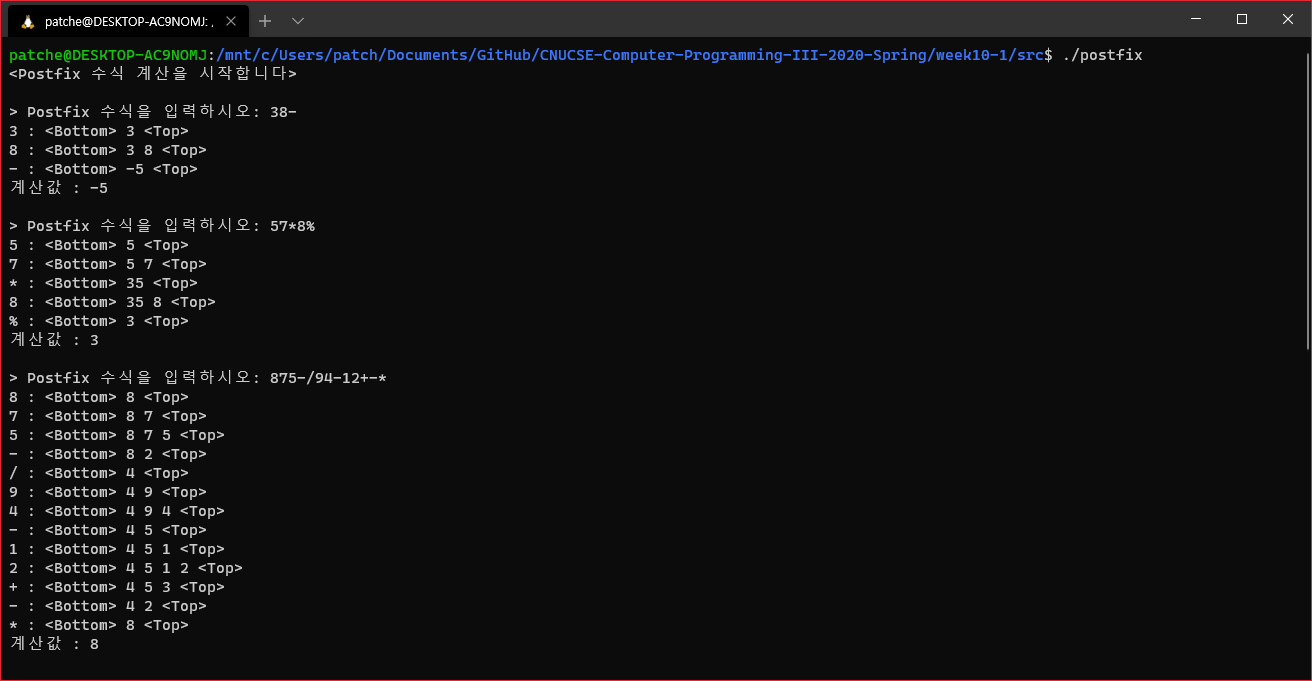
\includegraphics[width=\textwidth]{result_1.png}
                \caption{자료 제시 입력 실행결과 1}
                \label{}
            \end{figure}
            \begin{figure}[!htb]
                \centering
                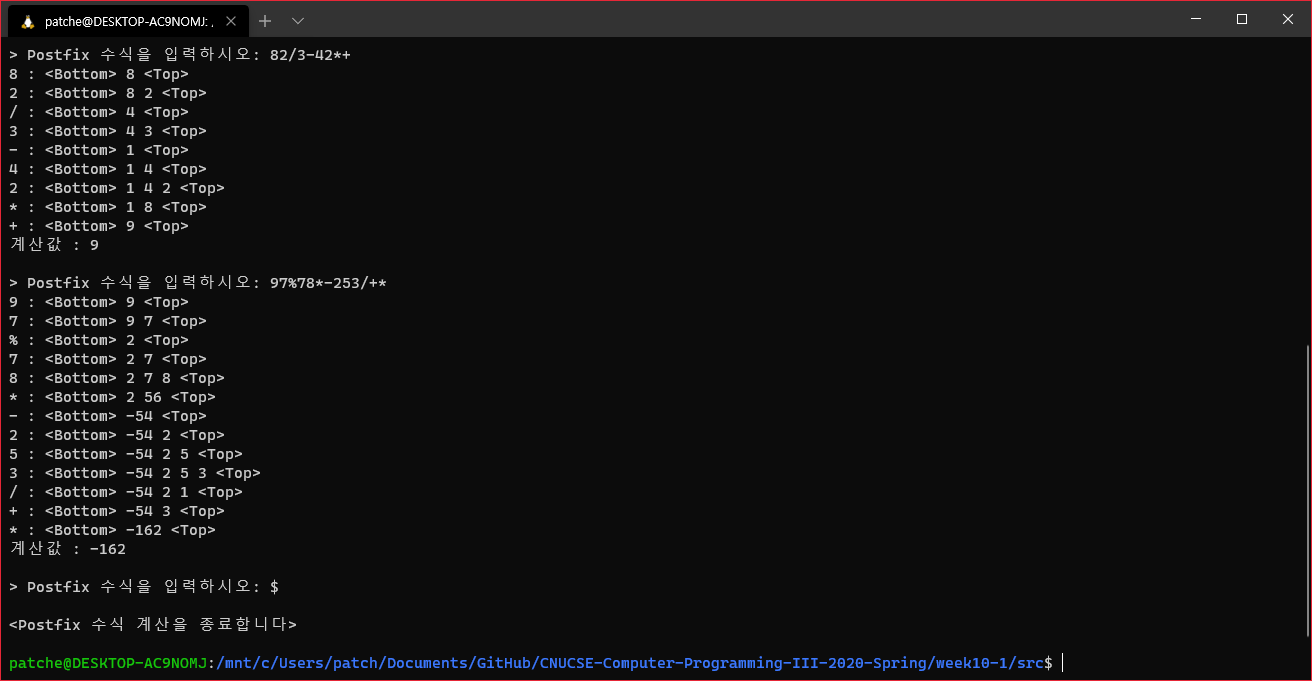
\includegraphics[width=\textwidth]{result_2.png}
                \caption{자료 제시 입력 실행결과 2}
                \label{}
            \end{figure}
        }

        \newpage

        \paragraph{%
            \begin{figure}[!htb]
                \centering
                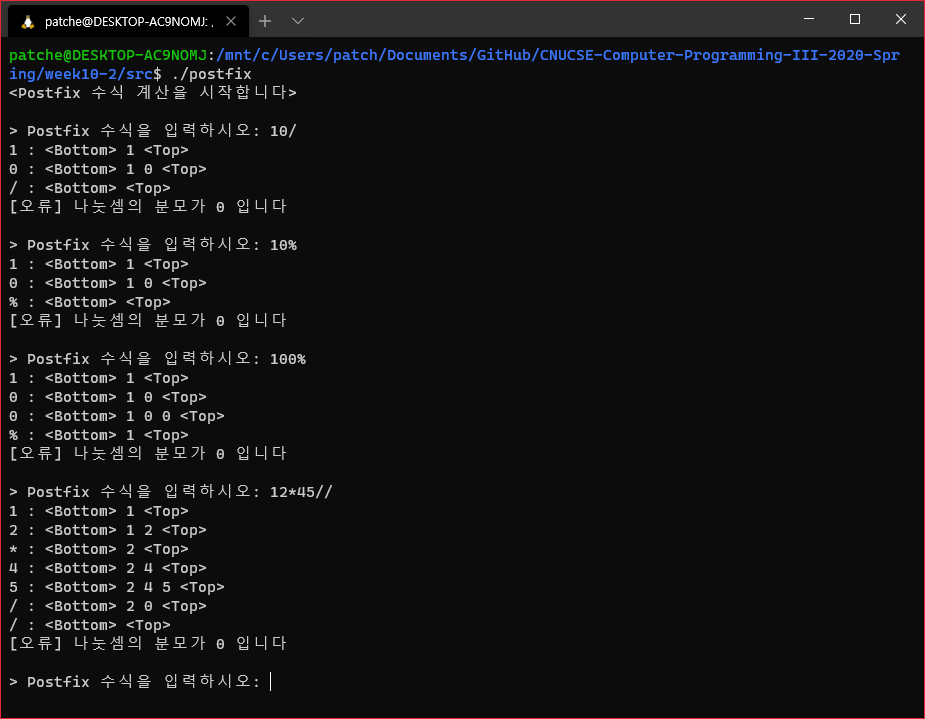
\includegraphics[width=\textwidth]{result_3.png}
                \caption{삭제 및 용량 초과시 실행 결과 1}
                \label{}
            \end{figure}
        }

        \newpage

        \paragraph{%
            \begin{figure}[!htb]
                \centering
                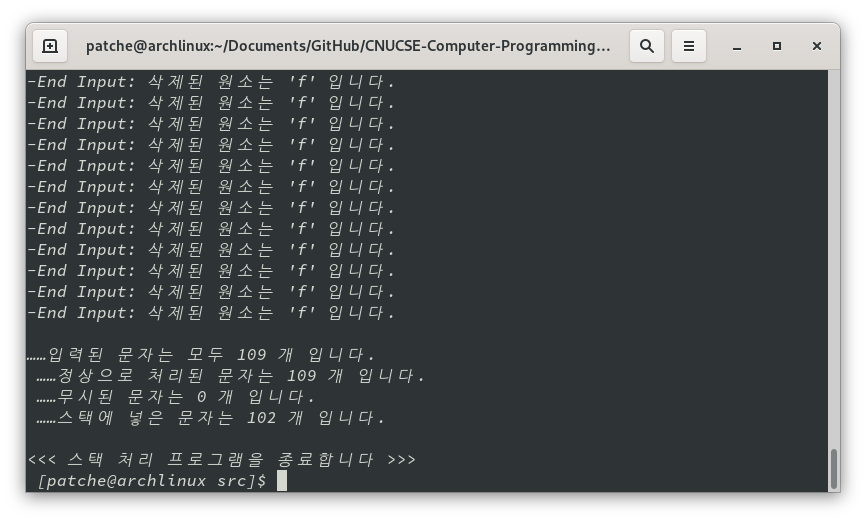
\includegraphics[width=\textwidth]{result_4.png}
                \caption{삭제 및 용량 초과시 실행 결과 2}
                \label{}
            \end{figure}
        }

        \newpage

        \section{입력과 출력}
            실습 자료에서 제시된 입력을 사용하였으며 출력 결과는 상기한 것과 같았음.
        \section{결과 분석}
            모든 입력에 대하여 정상적인 출력을 확인하였음.

    \chapter{소스코드}
        소스코드는 제출된 압축파일에 같이 동봉되어있으며 GitHub (0x00000FF/CNUCSE-Computer-Programming-III-2020-Spring) 에서도 열람할 수 있다.
\end{document}